\documentclass[autodetect-engine,dvi=dvipdfmx,ja=standard,
               a4j,11pt]{bxjsarticle}
\RequirePackage{geometry}
\geometry{reset,paperwidth=210truemm,paperheight=297truemm}
\geometry{hmargin=25truemm,top=20truemm,bottom=25truemm,footskip=10truemm,headheight=0mm}
\usepackage{graphicx}
\usepackage{fancyvrb}
\usepackage{amsmath}
\renewcommand{\theFancyVerbLine}{\texttt{\footnotesize{\arabic{FancyVerbLine}:}}}
\usepackage{newfloat}
\DeclareFloatingEnvironment[name=Listing, fileext=lol]{eopcode}
%%======== レポートタイトル等 ======================================%%
% ToDo: 提出要領に従って,適切なタイトル・サブタイトルを設定する
\title{中2 理科 一学期末 予想問題}

% ToDo: 自分自身の氏名と学生番号に書き換える
\author{}

% ToDo: レポート課題等の指示に従って適切に書き換える
\date{作成年: 2025年\\}  % 注:最後の\\は不要に見えるが必要.


%%======== 本文 ====================================================%%
\begin{document}
\maketitle
\section{\textbf{次の問いに答えなさい.(1) ~ (6)の化学式を書きなさい}【各2点】}
    (1) 水素と酸素の反応($\mathrm{H_2O}$)\\\\

    (2) 鉄と硫黄の反応($\mathrm{FeS}$)\\\\

    (3) 塩素と銅の反応($\mathrm{CuCl_2}$)\\\\

    (4) 塩化銅の分解($\mathrm{CuS} $)\\\\

    (5) 炭酸水素ナトリウムの分解($\mathrm{NaHCO_3}$)\\\\

    (6) マグネシウムの酸化($\mathrm{MgO} $)\\\\
    \clearpage
%%============================================================%%12点
\section{物質の成り立ち【各3点】}
\begin{figure}[htb]
        \centering
        \rotatebox{0}{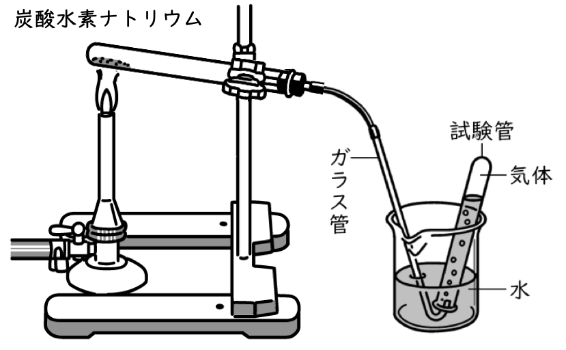
\includegraphics[scale=0.3]{熱分解炭酸水素ナトリウム.png}}
        \vspace{20pt} % ← 適宜調整
        \caption{}
\end{figure}
    (1) この実験で発生した気体は石灰水を加えてよく振ると白く濁った.何の気体だと考えられるか.\\\\

    (2) 実験後試験管の内側に液体がついていた.この液体に青い塩化コバルト紙をつけると何色に変化するか.\\\\

    (3) 試験管に残った物質は何か.\\\\

    (4) 炭酸水素ナトリウムと試験管に残った物質どちらの方が水に溶けやすいか\\\\

    (5) 炭酸水素ナトリウムと試験管に残った物質,それぞれ水に溶かして水溶液にした.その水溶液にフェノールフタレイン溶液を加えたとき,
    どちらの方が濃い赤色になるか.\\\\

    (6)この実験のように,元の物質とは違う物質ができる変化のことを何というか.\\\\

    (7) この実験において加熱をやめる前に試験管を水槽の水から抜く必要がある.それはなぜか\\\\

    (8) この実験において試験管の口を少し下げているのはなぜか.\\\\

    \clearpage
%%============================================================%%36点
\section{物質の成り立ち2【各3点】}
\begin{figure}[htb]
        \centering
        \rotatebox{0}{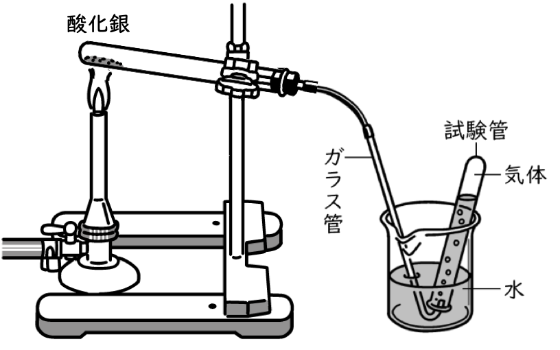
\includegraphics[scale=0.3]{酸化銀熱分解.png}}
        \vspace{20pt} % ← 適宜調整
        \caption{}
\end{figure}
    (1) この実験で発生した気体に,火のついた線香を近づけた.どうなるか\\\\

    (2) 加熱後の試験管に残っている物質は何か.\\\\

    (3) (2)の物質について正しいものすべてを選べ.完答
    \begin{itemize}
        \item [ア]  薬さじでこすると特有の光沢が出る\\
        \item [イ]  電気を通さない\\
        \item [ウ]  たたくと薄く伸びて広がる\\\\
    \end{itemize}
    

    (4) この実験のように一つの物質が,二つ以上の物質に分かれる化学変化を何というか.\\\\

    (5) 熱することで起こる(4)を特になんというか.\\\\

    (6)試験管の中の物質は加熱の前と後で重さはどう変化したか.\\\\
    \clearpage
%%============================================================%%54点
\section{物質の成り立ち3【各3点】}
\begin{figure}[htb]
        \centering
        \rotatebox{0}{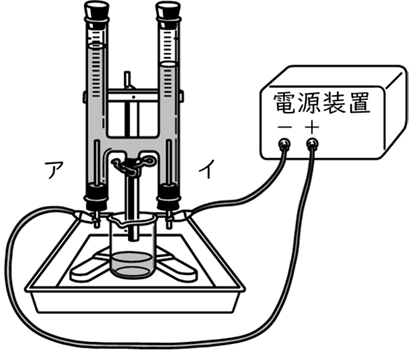
\includegraphics[scale=0.3]{水酸化ナトリウム電気分解.png}}
        \vspace{20pt} % ← 適宜調整
        \caption{}
\end{figure}
水に水酸化ナトリウムを溶かし,電流を流したところどちらの電極からもきたいがはっせいした.\\\\

    (1)水に水酸化ナトリウムを溶かした理由を述べよ\\\\

    (2)電極 ア に火のついた線香を近づけたところ炎をあげて激しく燃えた.何の気体かであると考えられるか.\\\\

    (3)電極アは陽極陰極どちらか.\\\\

    (4)電極イからはどのような気体が発生すると考えられるか.\\\\

    (5)電源装置の + につながっているのは電極ア,イのどちらか.\\\\

    (6)この実験において水に起きた化学変化をかけ.\\\\

    (7)この実験のように,電流を流すことで物質を分解することを何というか.\\\\
    \clearpage
%%============================================================%%75点
\section{物質の法則【各3点】}
\begin{figure}[htb]
        \centering
        \rotatebox{0}{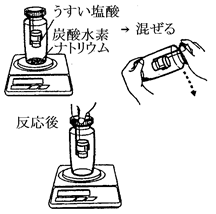
\includegraphics[scale=0.7]{密閉容器化学変化.png}}
        \vspace{20pt} % ← 適宜調整
        \caption{}
\end{figure}
    (1) 混ぜると気体が発生したこの物質は何か.\\\\

    (2)この実験の化学変化を,化学反応式で表せ.\\\\

    (3)反応前と反応後で全体の質量はどう変化したか.\\\\

    (4)(3)であることを何の法則というか\\\\
\clearpage

  \begin{figure}[htb]
        \centering
        \rotatebox{0}{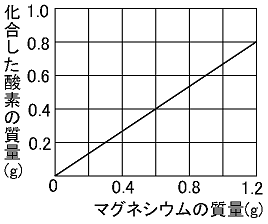
\includegraphics[scale=0.7]{酸素マグネシウムグラフ.png}}
        \vspace{20pt} % ← 適宜調整
        \caption{}
\end{figure}  
 (1)1.2gのマグネシウムと結合した酸素は何グラムか.\\\\\\

 (2)0.6gのマグネシウムからできる酸化マグネシウムは何グラムか\\\\\\

 (3)マグネシウムと酸化マグネシウムの比を答えなさい.   \\\\\\
 %%=========================================================96点

 \section{温度変化を伴う反応【各2点】}
 袋に炭酸水素ナトリウムをいれ温度を図り,クエン酸を加えた.\\\\\\
 
 (1)この袋に水を加えてよく振ると温度はどうなるか.\\\\\\

 (2)よく振るとある気体が発生したそれは何か.\\\\\\
%%============================================================%%
\end{document}
%%============================================================%%

\begin{Verbatim}
\end{Verbatim}
\begin{table}b\begin{figure}[htb]
        \centering
        \rotatebox{0}{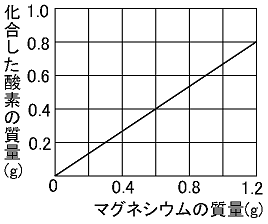
\includegraphics[scale=0.7]{酸素マグネシウムグラフ.png.png}}
        \vspace{20pt} % ← 適宜調整
        \caption{}
\end{figure}
    \centering 
      \caption{計算結果}%表の題%
      \begin{tabular}{|l|l|l|}
      \hline
        \textbf{} & \textbf{} & \textbf{} \\ %label
      \hline
        \verb||    &   $1$  &   $1$  & \\
      \hline
      \end{tabular}
    \end{table}
    \begin{figure}[htb]
        \centering
        \rotatebox{270}{\includegraphics[scale=0.4]{Pro_Lan_Result.PNG}}
        \vspace{20pt} % ← 適宜調整
        \caption{}
    \end{figure}
\section{作成したプログラムのソースコード}
\begin{Verbatim}[numbers=left, xleftmargin=8mm, numbersep=6pt,
    fontsize=\small, baselinestretch=0.8]
\end{Verbatim}
